\section{Database Structure}
\label{sec:databasestructure}

We distinguish between two parts of the database, the login part, and the model part. 
The model part is created from our Model \ref{sub:modelComponent} using the ADO.NET Entity Framework(EF) which is described in subsection \ref{sub:adonet}. 
We choose to use ADO.NET EF because we do not have to worry about converting our tuples to objects and to make sure that changed properties are mapped to the database correctly.  
To administrate users we use the inbuilt ASP.NET membership provider which provides a login system with support for role authorization. 
We use this provider since it saves time instead of building our own login system. 
Security is not a big concern in this project and therefore we do not want to spend time creating a secure login system. 
The major disadvantage is that including the membership providers database scheme with the model is not supported and does not work properly. 
Therefore we had to add a person entity and change the register functionality to also save the registered person in our person table. 
This gives some redundant data, but only the username and email. 
When we needs to access data from the membership tables we had to use SQL statements and not the object oriented approached we used for the rest. 
This is limited since our main functionality depends on the model. 

\subsection{ADO.NET Entity Framework}
\label{sub:adonet}
The ADO.NET is designed by Microsoft with the purpose of making a disconnected database architecture to use with the .NET framework \cite{adonetDesignGoal}. 
This architecture is an improvement from the older database architectures where a connection were made and held open in the entire runtime. With a disconnected database the connection is only open when data is needed \cite{disconnectedData}. 

The ADO.NET EF is an object relational mapping framework \cite{adonetEntityFramework} build upon ADO.NET. 
Together with the ADO.NET Entity Data Model Designer and a SQL Server ADO.NET EF gives a strong tool for mapping a database and using the data in a object oriented matter, without dealing with the transformation from entity to class and from tuple to object. 
The Designer is built into Visual Studio Ultimate. 

Using the ADO.NET and the Entity Data Model Designer can be done in two ways. 
The  model can be created from an already existing database or by creating the model and generate a database from this \cite{adonetEntityDataModelDesigner}.
We use the last approach and created the database from the model. 
In this way we do not have to worry about setting the right foreign keys and relational tables. Instead we get a fully functional model linked to a database. 

Our model as it is in the ADO.NET Entity Model Designer is shown on figure \ref{fig:edmxModel}
\begin{figure}[htb]
	\centering
		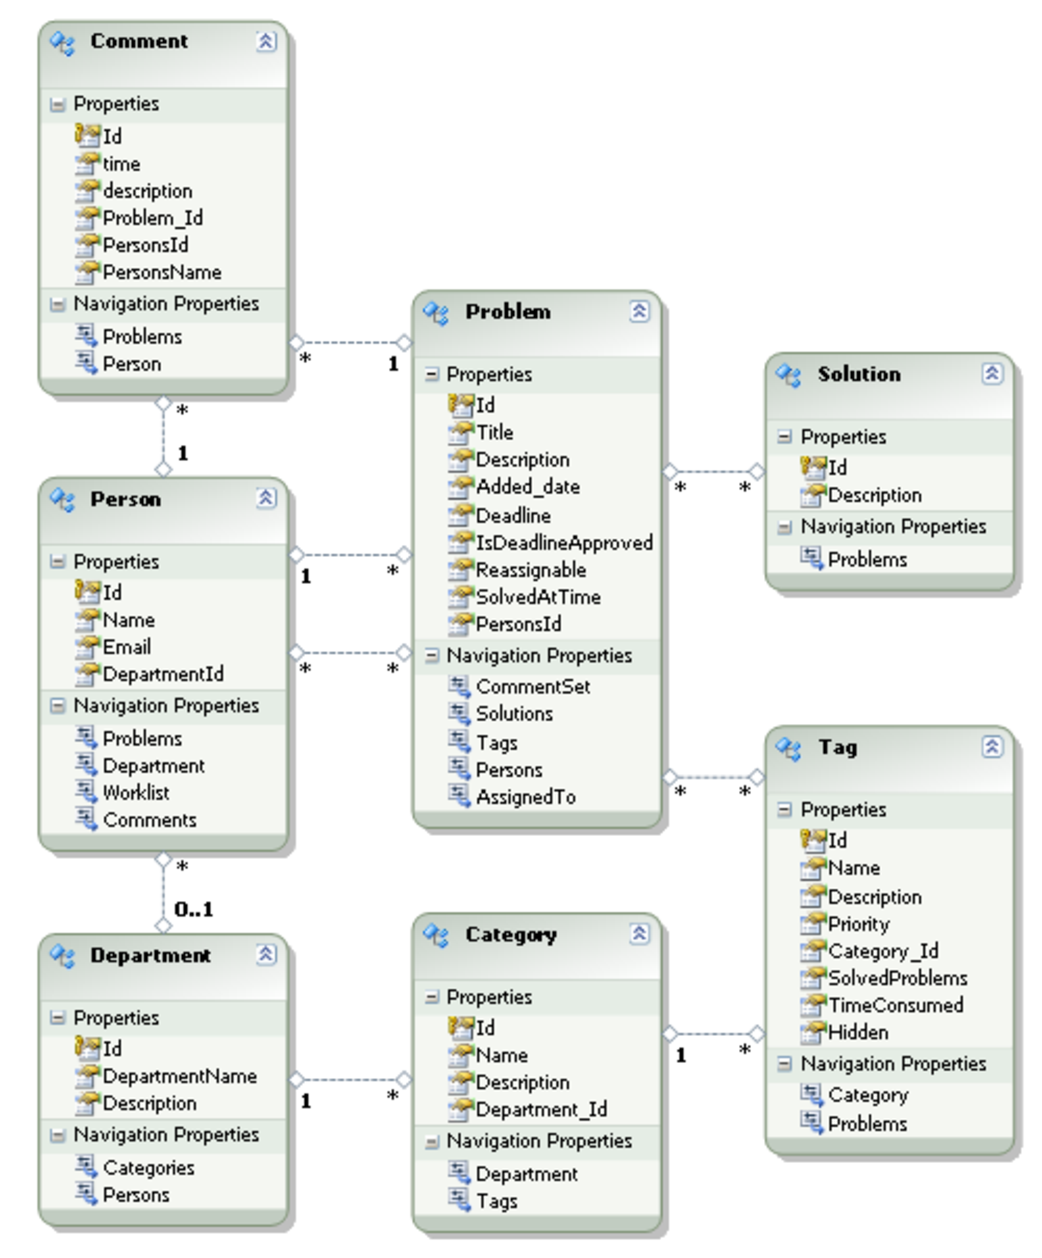
\includegraphics[scale=0.7]{input/implementation/mvc/Model.pdf}
	\morscaption{Our model as it is seen in the ADO.NET Entity Data Model Designer.}
	\label{fig:edmxModel}
\end{figure}

